\documentclass[12pt, a4paper]{article}
\usepackage{graphicx}
\usepackage[slovenian]{babel}
\usepackage{csquotes}
\usepackage{biblatex}
\usepackage{amsmath}
\usepackage{float}
\addbibresource{porocilo.bib}
\graphicspath{{images/}}
\title{Žarko - upodabljanje s sledenjem žarkov}
\author{Filip Trplan}
\date{Avgust 2025}

\begin{document}
\maketitle

\begin{figure}[h]
	\centering
	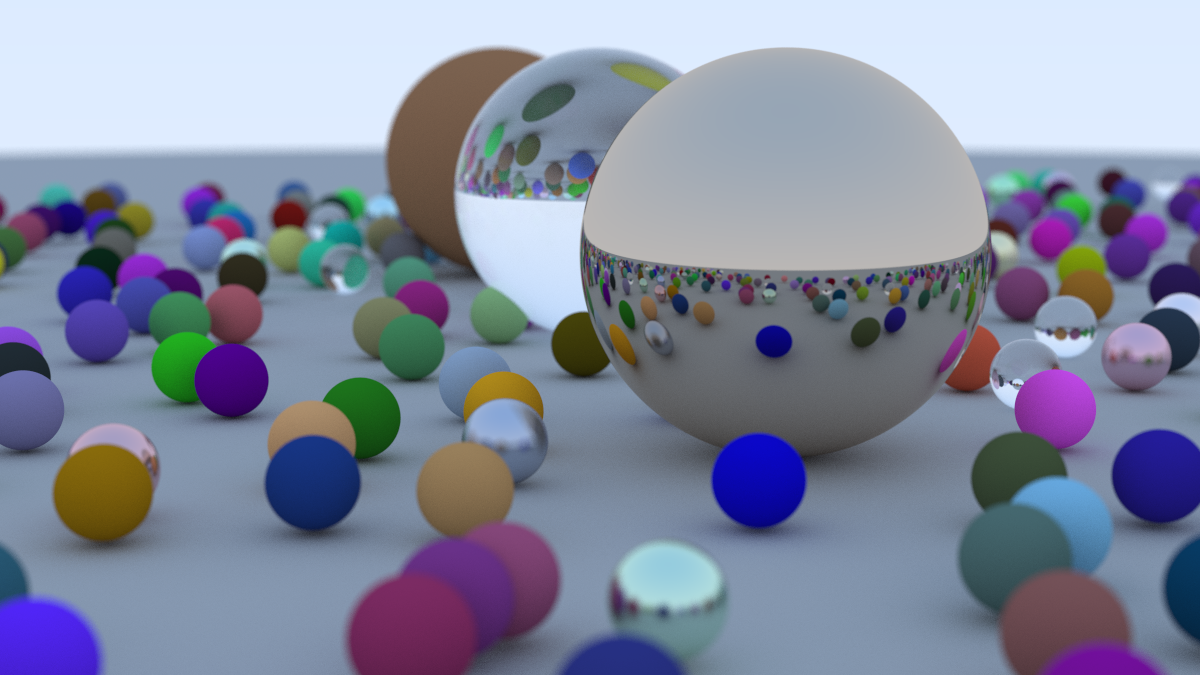
\includegraphics[width=\textwidth]{cover}
	\caption{Končni rezultat}
\end{figure}

V temu poročilu bom predstavil tehniko upodabljaljanja (\textit{rendering}) s sledenjem žarkov
(\textit{ray tracing}). Lotil se bom prvo osnov sledenja žarkov in bom nato prešel na ustvarjanje treh
različnih tipov materialov ter končal z simulacijo globinske ostrine (\textit{depth of field}).

Vseskozi poročila se zgledujem po knjigi \textit{Ray Tracing in One Weekend} \cite{Shirley2025RTW1}

\section{Osnove sledenja žarkov}

Osnovna ideja upodabljanja s sledenjem žarkov je, da si predstavljamo prikazano sliko kot ploskev in kamero
orientirano v 3D prostoru. V realnem svetu svetloba izvira iz svetlobnih virov kot so sonce ali luči in se
nato odbije od raznih objektov dokler ne doseže našega očesa oz. senzorja na kameri. Ker pa veliko teh žarkov
zgreši našo kamero, bomo obrnili smer žarkov in jih bomo izstrelili iz kamere.

Žarek bo potoval iz kamere skozi piksel našem vidnem oknu (\textit{viewport}) ter se nato odbil po
virtualnem svetu dokler ne bo dosegel svetlobnega vira (v našem primeru bo to nebo).

\begin{figure}[H]
	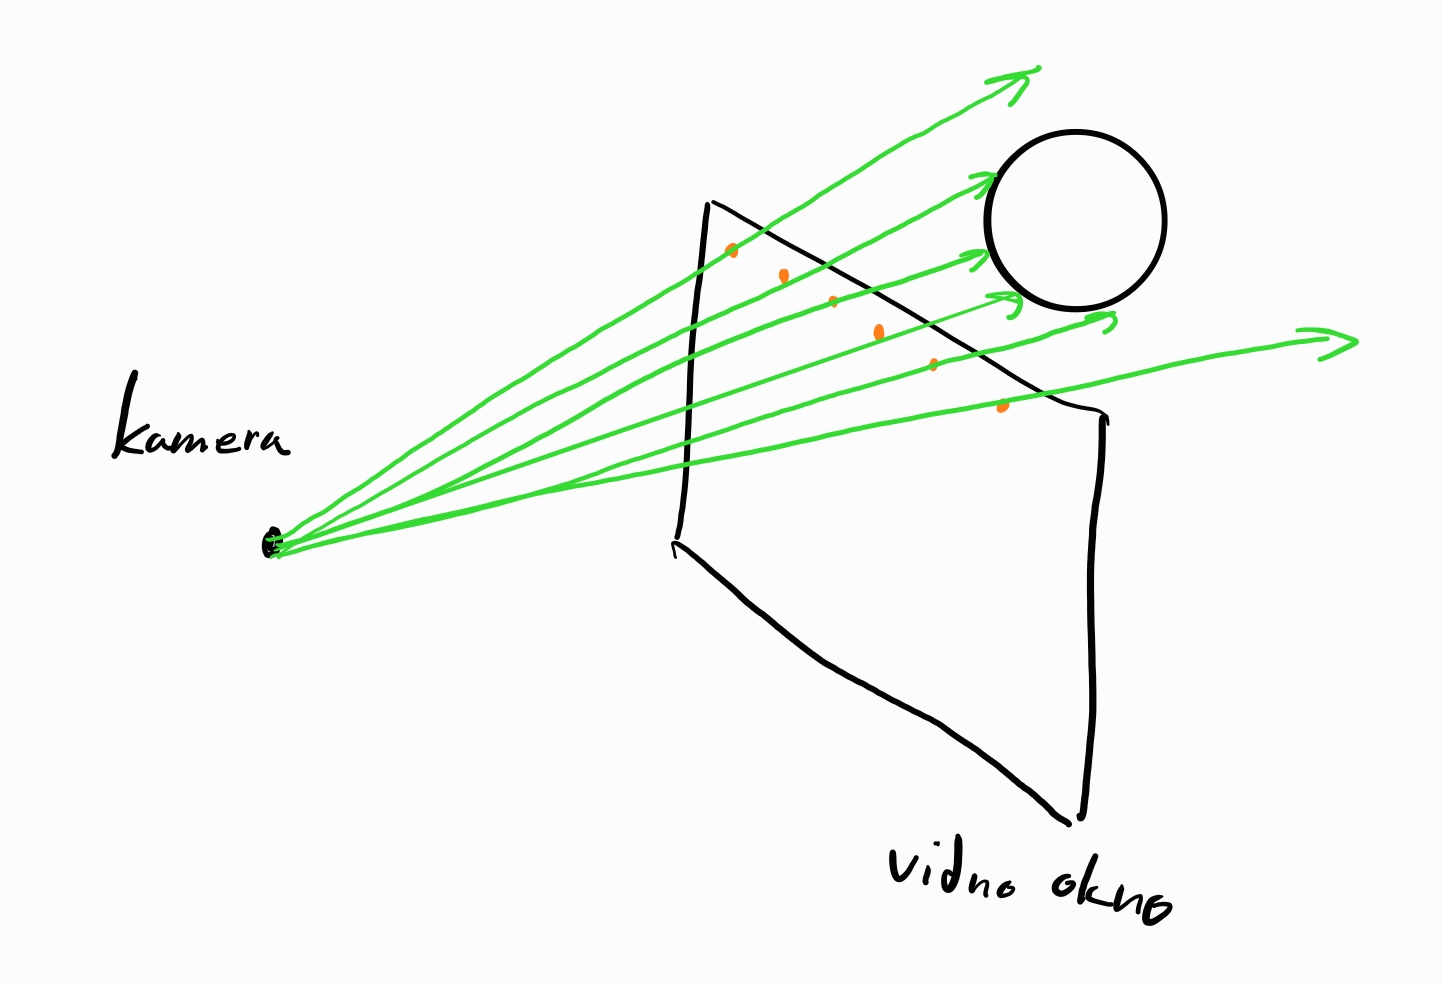
\includegraphics[width=\textwidth]{shema_zarki}
	\caption{Shema sledenja žarkov}
\end{figure}

Vpeljimo par oznak, da si bomo lažje predstavljali kako te žarki potekajo. Pozicijo kamere bomo imenovali $C$,
levi zgornji piksel bo $P_{00}$ in če so piksli na mreži, bodo enakomerno razporejeni tako da bo v horizontalni
smeri jih ločil vektor $\Delta u$ in v vertikalni $\Delta v$. Prikazane so na sliki \ref{fig:oznake}.

\begin{figure}[h]
	\centering
	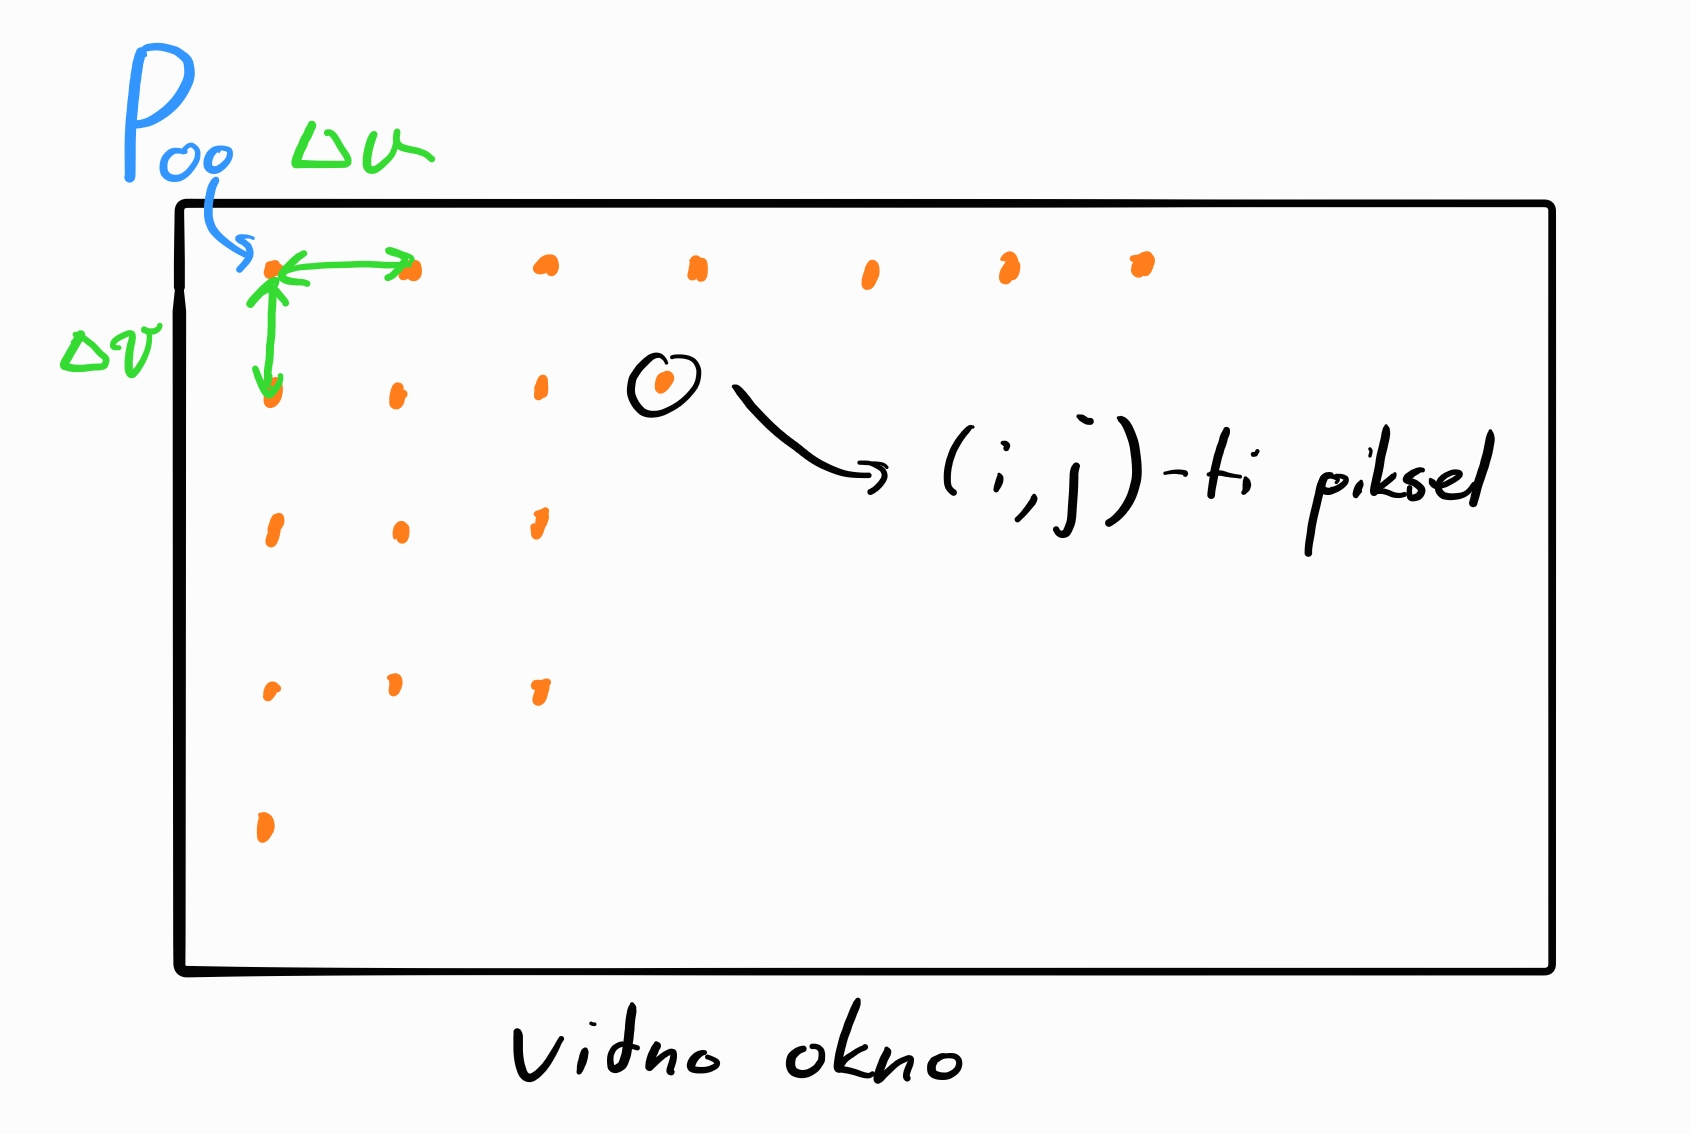
\includegraphics[width=\textwidth]{vidno_okno}
	\caption{Oznake prikazane vizualno}
	\label{fig:oznake}
\end{figure}

Potem lahko žarek $\vec{r}$, ki potuje skozi piksel $(i,j)$ parametriziramo s $t$:

\begin{equation}
	\vec{r} = C + t \cdot (P_{00} + i \cdot \Delta u + j \cdot \Delta v - C)
\end{equation}

V prihodnje pa bomo obravnavali splošne žarke z izvorom v $O$ in smerjo $\vec{d}$.

\section{Detekcija trka}

Trenutno naši žarki samo streljajo v praznino zato bomo zdaj v svet dodali objekte v katere lahko žarki trčijo.
Matematično je najlažje opisati sfero. Splošna enačba za sfero s središčem $C$ in radijem $r$ je

\begin{equation}
	\label{eq:sfera}
	(C_{x} - x)^2  + (C_{y} - y)^2  + (C_{z} - z)^2  = r^2
\end{equation}

Če točko $(x,y,z)$ označimo kot $P$ lahko \ref{eq:sfera} zapišemo kot skalarni produkt.

\begin{equation}
	(C - P)(C - P) = r^2
\end{equation}

Naša točka pa leži na žarku torej dobimo

\begin{equation}
	(C - (O + t \vec{d}))(C - (O + t \vec{d})) = r^2
\end{equation}

Po nekaj preurejanja enačbe dobimo naslednjo kvadratno enačbo

\begin{equation}
	t^2 \lVert C \rVert ^2  - 2 t \cdot \vec{d} (C - O) + \lVert C - O \rVert ^2  - r^2 = 0
\end{equation}

S pomočjo diskriminante lahko zlahka preverimo ali naš žarek sploh zadane sfero. Če rešitev obstaja pa vzamemo
najmanjšo pozitivno (torej najbližjo kameri v smeri pogleda). V primeru, da pozitivna rešitev ne obstaja pa
smatramo, kot da žarek ni zadel objekta, saj je za kamero.

Na sliki \ref{fig:red_sphere} vidimo primer izrisa sfere, kjer jo samo obarvamo samo z rdeco barvo.

\begin{figure}[H]
	\label{fig:red_sphere}
	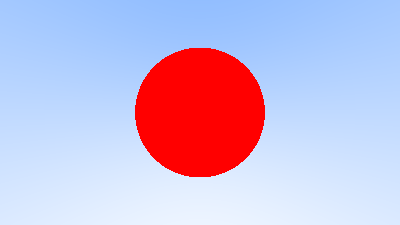
\includegraphics[width=\textwidth]{red_sphere}
	\caption{Rdeče obarvana sfera}
\end{figure}

Na zgornji sliki vidimo, da ima sfera zagast rob. To se zgodi zaradi diskretizacije pikslov v mrežo. Temu
pojavimo pravimo \textit{aliasing}. Znebimo se ga tako, da za vsak piksel izstrelimo več žarkov ki so naključno
pertrubirani za največ polovično razdaljo med piksli, ter nato barvo teh žarkov povprečimo. Tehnika se imenuje
MSAA (\textit{multisample anti-aliasing}) in smo jo izbrali, ker je v kontekstu sledenja žarkov najbolj
enostavna za implementirati.

\section{Materiali}

\subsection{Difuzni materiali in Lambertov odboj}

Prve materiali, ki se jih bomo lotili so difuzni. Taki materiali v realnem svetu zgledajo mat in so takega
videza, ker se žarki naključno odbijejo od površine objekta. Lambertov odboj je aproksimacija takih materialov,
ki pravi, da naj je smer odbitega žarka izbrana sorazmerno s količino $\cos (\phi) $, kjer je $\phi$ vpadni
kot.

\begin{figure}[H]
	\centering
	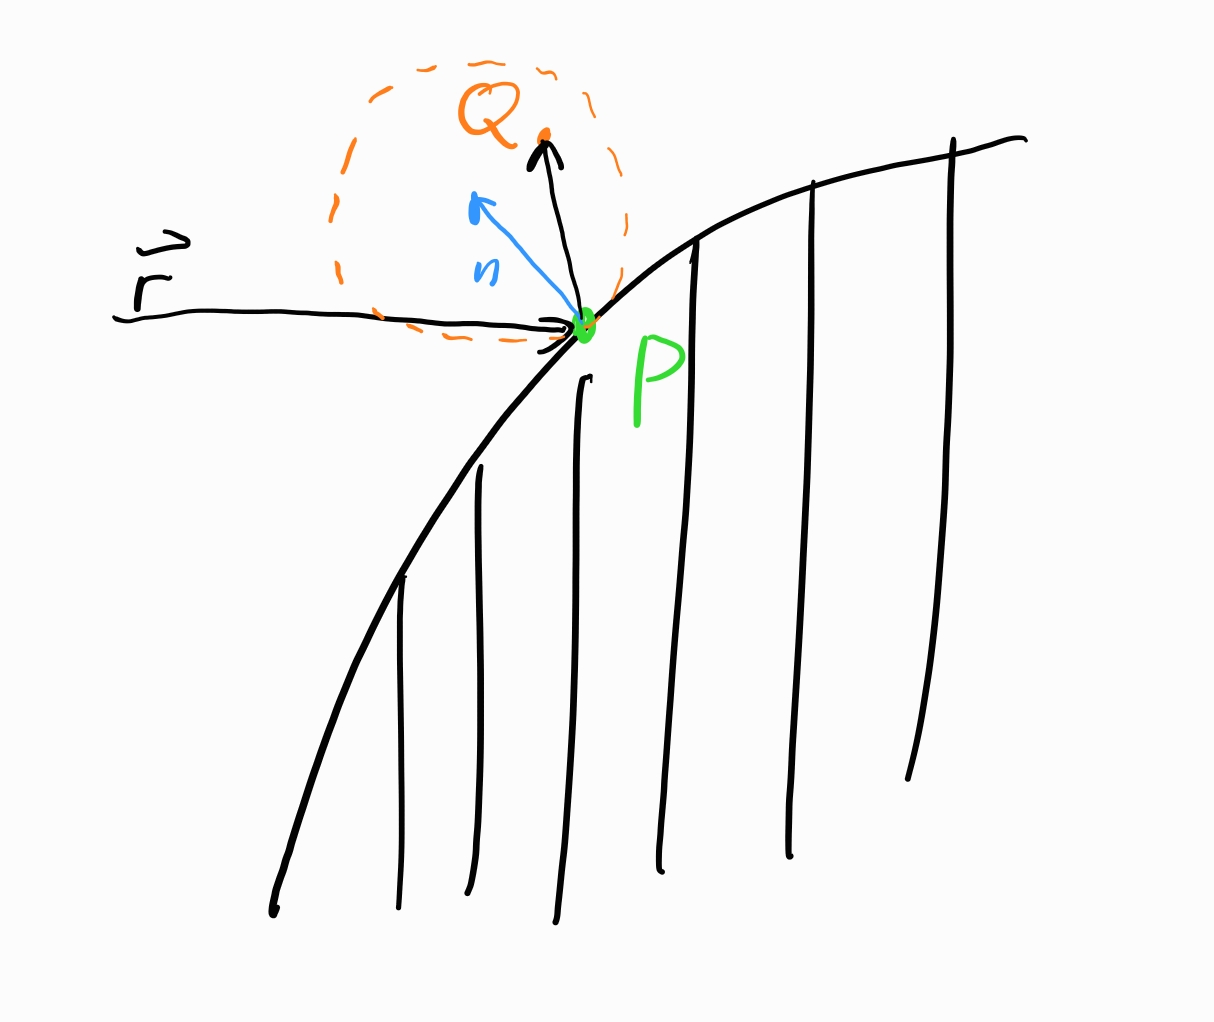
\includegraphics[height=250pt]{shema_difzuni}
	\caption{Lambertov odboj}
\end{figure}

Če žarek seka objekt na točki $P$ in je normala površine vektor $n$, potem izberemo naključno točko $Q$
znotraj enotske sfere s središčem $P + n$ (kjer je normala enotski vektor). Smer odbitega žarka je potem
$Q - P$.

\begin{figure}[H]
	\centering
	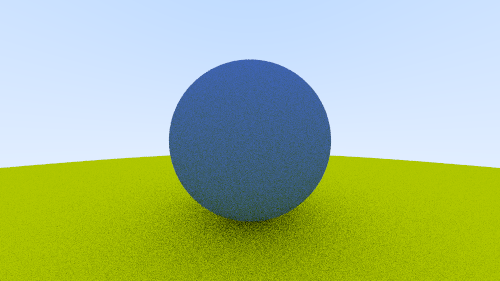
\includegraphics[width=400pt]{difuzni}
	\caption{Dve difuzni sferi}
\end{figure}

Da dodamo barvo, odbiti žarek pomnožimo z barvo objekta, ki ji pravimo \textit{albedo}. Tako se barva
svetlobnega vira postopoma spreminja ob vsakem odboju - množi se z albedo vsakega objekta, s katerim se
žarek sreča. Končna barva piksla je zato produkt barve svetlobnega vira in vseh albedo vrednosti
objektov na poti žarka.

\textit{Opomba: }, ker se ta metoda zanaša na naključne procese za aproksimacijo realnega sveta (Monte Carlo),
dobimo nekaj šuma v sliki.

\subsection{Kovinski materiali}

Kovine imajo svojo barvo, vendar pa hkrati tudi odbijejo del svetlobe pod istim kotom, kot je
žarek srečal objekt. Odbiti žarek je sestavljen iz dveh delov: zrcaljeni del in t.i. zamegljeni del
(\textit{fuzziness}). Končni odbiti žarek je vsota teh dveh vektorjev.

\begin{figure}[H]
	\centering
	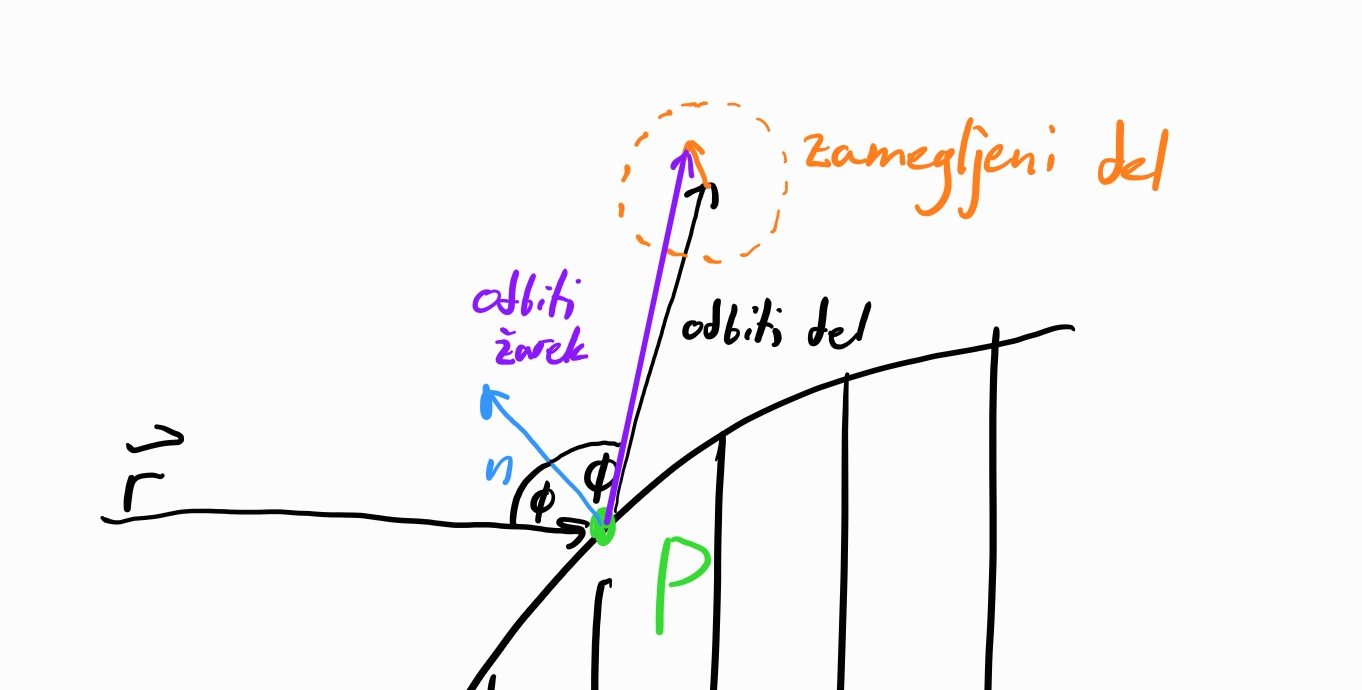
\includegraphics[width=400pt]{metal}
	\caption{Odboj žarka od kovinskega materiala}
\end{figure}

Zrcaljeni del je preprosto vpadni žarek zrcaljen čez ploskev, ki jo opiše normala in z zamenjano smerjo.
Zameglejni del pa simulira hrapavost kovine in je samo naključni vektor znotraj enotske sfere pomnožen
s parametrom $0 \leq f \leq 1$, ki kontrolira kako zamegljen je objekt.

\subsection{Dielektrični materiali}
Še zadnja vrsta materialov, ki jih uporabljamo, so prosojni materiali oziroma dielektriki. To so na primer voda,
steklo in diamant. Ko svetloba preide skozi te materiale se upogne, ko prehaja med dvema materialoma z
različnima lomnima količnikoma. Na primer, zrak ima količnik blizu 1, steklo pa okoli 1,5. Lom svetlobe opisujemo
z lomnim zakonom.

$$
	tukaj zakon
$$

% tukaj bom dal se diagram zakona

Lomni zakon ni vedno rešljiv — pri prevelikem vpadnem kotu nastopi popolni notranji odboj — svetloba se v takem
primeru v celoti odbije od meje med materialoma, namesto da bi prešla v drugi medij. Tudi ce je enacba resljiva
pa se svetloba ne lomi v celoti, nek delez se vedno odbije od materiala. Ta pojav opisujejo Fresnelove enacbe, ki
so odvisne od vpadnega kota. Ker pa je resevanje tega sistema pocasno, v praksi uporabimo polinomsko Schlickovo
aproksimacijo

$$
	schlickova aproksimacija
$$

Torej v praksi bomo uporabljali Monte Carlo metodo, kjer se žarek odbije od površine materiala, če lomni zakon
ni rešljiv ali pa velja $naključno število < Schlickova aproksimacija$.

\section{Globinska ostrina}

V pravi kameri je leča sestavljena iz več steklenih elementov, ki so za odprtino, ki ji pravimo zaslonka.
Zaradi tega, ker je ta odprtina večja od točke, bodo objekti na določeni razdalje povsem ostri, ostali pa
zamegljeni. Temu pojavu pravimo globinska ostrina. Namesto modeliranja kompleksnega sistema večih elementov
pa bomo uporabili model tanke leče.

% skica tanke lece in zakaj zarki niso ostri

Efekt bomo simulirali tako, da se bomo pretvarjali, da je pozicija naše kamere v resnici pozicija leče in
da je položaj našega vidnega okna ravnina, kjer bodo objekti izostreni.

Kako to dosežemo? Izhodišča žarkov naključno zamaknemo za vektor, izbran v enotskem krogu, in ga skaliramo s
faktorjem, izračunanim glede na odprtost zaslonke. Ti žarki so nato usmerjeni točno v ciljni piksel na vidnem
oknu, vendar zaradi zamaknjenih izhodišč malo odstopajo od pričakovane poti pred in po oknu, kar ustvari učinek
globinske ostrine.

\printbibliography

\end{document}
